\documentclass[12pt,a4paper]{article}
\usepackage{ctex}
\usepackage{amsmath,amscd,amsbsy,amssymb,latexsym,url,bm,amsthm}
\usepackage{epsfig,graphicx,subfigure}
\usepackage{enumitem,balance}
\usepackage{wrapfig}
\usepackage{mathrsfs,euscript}
\usepackage[usenames]{xcolor}
\usepackage{hyperref}
\usepackage[vlined,ruled,linesnumbered]{algorithm2e}
\usepackage{array}
\hypersetup{colorlinks=true,linkcolor=black}

\newtheorem{theorem}{Theorem}
\newtheorem{lemma}[theorem]{Lemma}
\newtheorem{proposition}[theorem]{Proposition}
\newtheorem{corollary}[theorem]{Corollary}
\newtheorem{exercise}{Exercise}
\newtheorem*{solution}{Solution}
\newtheorem{definition}{Definition}
\theoremstyle{definition}

\renewcommand{\thefootnote}{\fnsymbol{footnote}}

\newcommand{\postscript}[2]
 {\setlength{\epsfxsize}{#2\hsize}
  \centerline{\epsfbox{#1}}}

\renewcommand{\baselinestretch}{1.0}

\setlength{\oddsidemargin}{-0.365in}
\setlength{\evensidemargin}{-0.365in}
\setlength{\topmargin}{-0.3in}
\setlength{\headheight}{0in}
\setlength{\headsep}{0in}
\setlength{\textheight}{10.1in}
\setlength{\textwidth}{7in}
\makeatletter \renewenvironment{proof}[1][Proof] {\par\pushQED{\qed}\normalfont\topsep6\p@\@plus6\p@\relax\trivlist\item[\hskip\labelsep\bfseries#1\@addpunct{.}]\ignorespaces}{\popQED\endtrivlist\@endpefalse} \makeatother
\makeatletter
\renewenvironment{solution}[1][Solution] {\par\pushQED{\qed}\normalfont\topsep6\p@\@plus6\p@\relax\trivlist\item[\hskip\labelsep\bfseries#1\@addpunct{.}]\ignorespaces}{\popQED\endtrivlist\@endpefalse} \makeatother

\begin{document}
\noindent

%========================================================================
\noindent\framebox[\linewidth]{\shortstack[c]{
\Large{\textbf{Lab08-Computational Complexity}}\vspace{1mm}\\
CS214-Algorithm and Complexity, Xiaofeng Gao, Spring 2019.}}
\begin{center}
\footnotesize{\color{red}$*$ If there is any problem, please contact TA Jiahao Fan or TA Mingran Peng.}

% Please write down your name, student id and email.
\footnotesize{\color{blue}$*$ Name:\underline{��ѩ��}  \quad Student ID:\underline{515030910347} \quad Email: \underline{13487426939@qq.com}}
\end{center}

\begin{enumerate}
    \item
    \begin{solution}
      The following is the process of solution.\\
      \textbf{a.} In this case, the set of state is $Q=\{q_{S},q_{1},q_{2},q_{3},q_{4},q_{H}\}$.\\
      we use $q_{1}$ to find $\Box$, then convert $q_{1}$ to $q_{2}$.  If  $q_{2}$ find 1 from left to right, then convert $q_{2}$ to $q_{3}$ and convert 1 to $\Box$, turn direction around.  If $q_{3}$ find 1 from right to left, then convert $q_{3}$ to $q_{2}$ and convert 1 to $\Box$, turn direction around, ; Repeat until $q_{2}$ find $\triangleleft$  then turn direction around, and convert $q_{2}$ to $q_{4}$, Then we use $q_{4}$ to find 1 and turn direction aroundp and convert $q_4$ to $q_H$.\\
     \color{red} Begin: use $q_1$ to find $\Box$, and convert $q_1$ to $q_2, q_2$ point to 1 on the left  of $\Box$. \color{black}\\
      $\langle q_S, \triangleright \rangle \rightarrow \langle q_1, \triangleright,  R\rangle$. \\
      $\langle q_1, 1 \rangle \rightarrow \langle q_1, 1,  R\rangle$. \\
      $\langle q_1, \Box \rangle \rightarrow \langle q_2, \Box,  R\rangle$.\\
      \color{red} Loop: use $q_2,q_3$ to convert 1 to $\Box$ one by one alternately. \color{black}\\
      $\langle q_2, \Box \rangle \rightarrow \langle q_2, \Box,  R\rangle$. \\
      $\langle q_2, 1 \rangle \rightarrow \langle q_3, \Box,  L\rangle$. \\
      $\langle q_3, \Box \rangle \rightarrow \langle q_3, \Box,  L\rangle$. \\
      $\langle q_3, 1 \rangle \rightarrow \langle q_2, \Box,  R\rangle$. \\
      \color{red} End: use $q_4$ to find  1 on the left  of $\Box$ and $p_4$ point to next cell.\color{black}\\
      $\langle q_2, \triangleleft, \rangle \rightarrow \langle q_4, \triangleleft,  L\rangle$.\\
      $\langle q_4, \Box \rangle \rightarrow \langle q_4, \triangleleft,  L\rangle$. \\
      $\langle q_4, 1,\rangle \rightarrow \langle q_H, 1,  R\rangle$. \\

      \textbf{b.}The state transition diagram in txf\_homework\_08.vsdx like following picture.
      \begin{centering}
      \begin{figure}[htbp]
      \begin{minipage}[h]{0.8\textwidth}
      \centering
      \hspace{3cm} 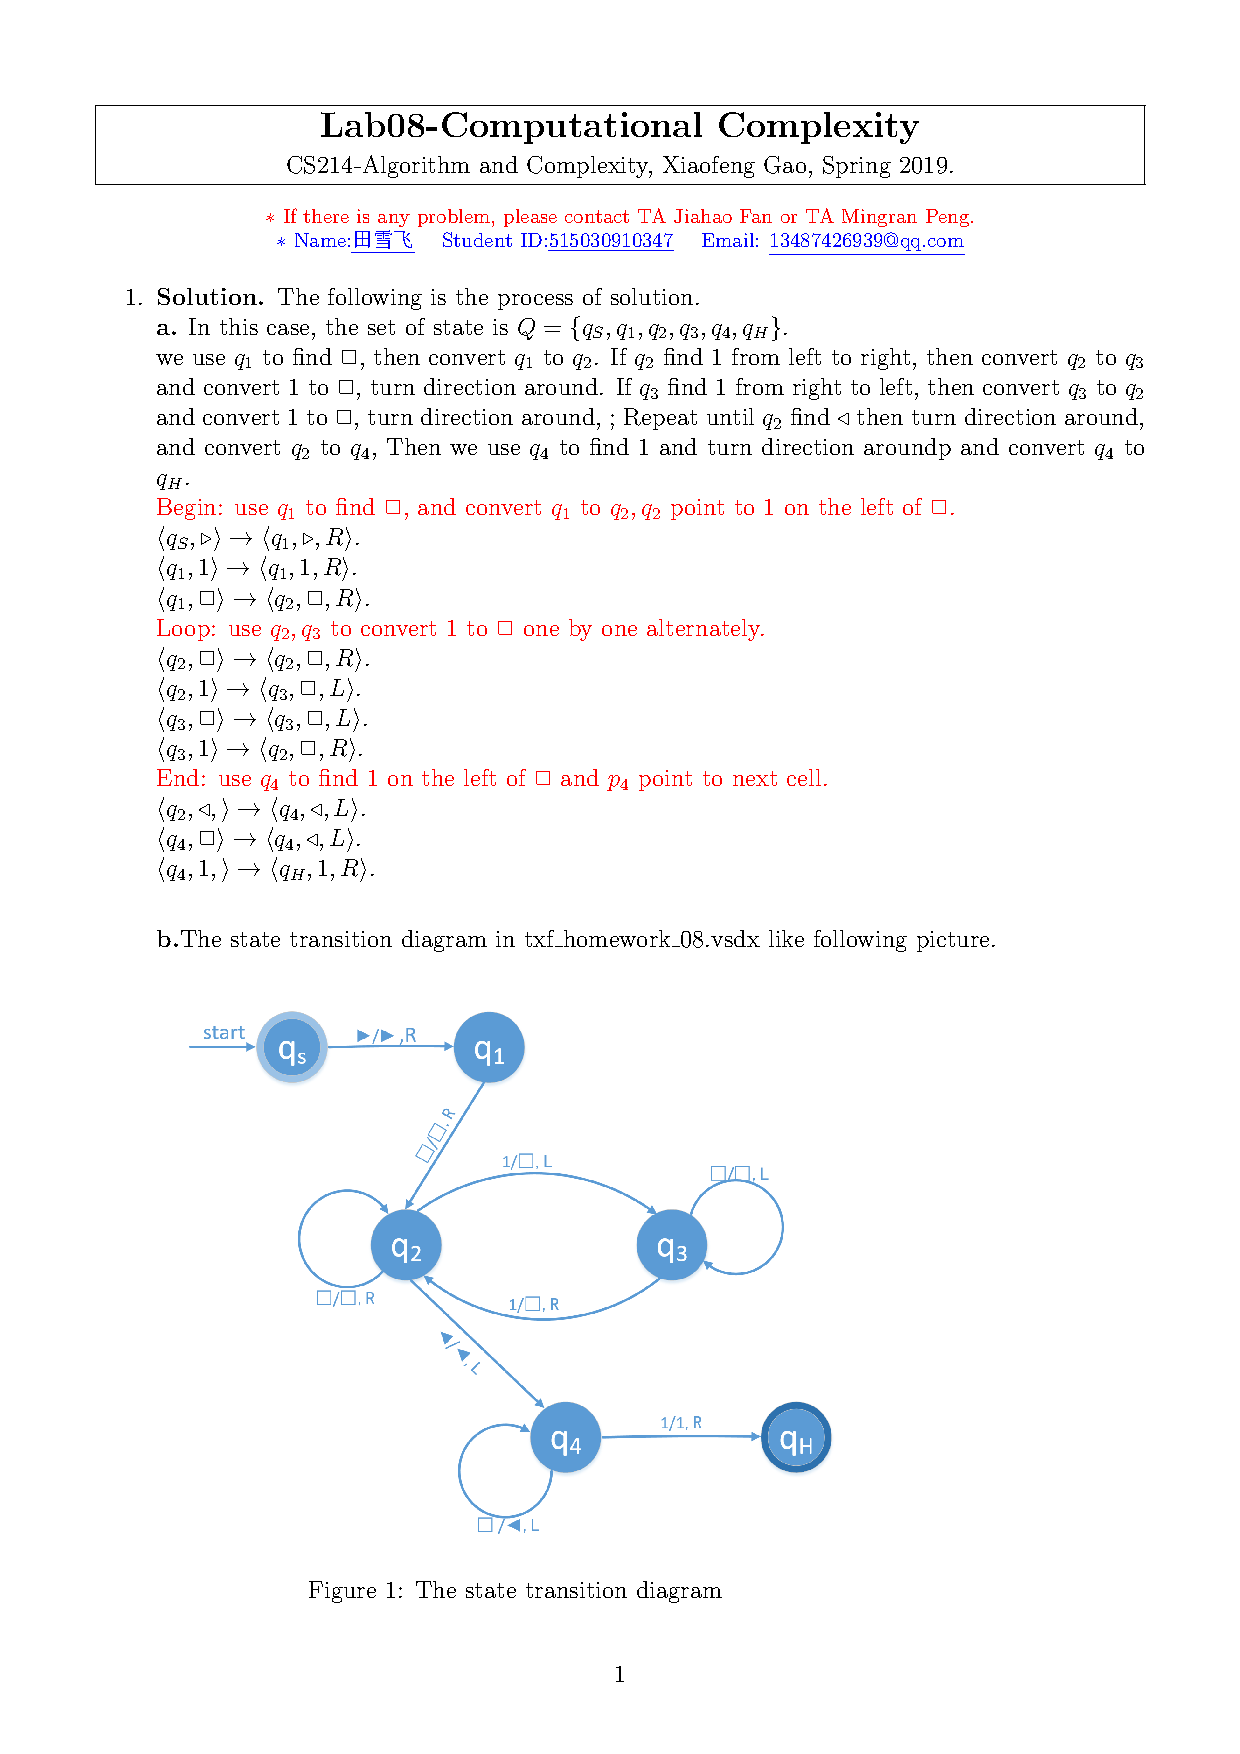
\includegraphics[width=0.9\textwidth]{txf_homework_08.png}
      \caption{The state transition diagram}
      \end{minipage}
      \end{figure}
        \end{centering}
        \\
        \textbf{c.}Whole process from initial to final configurations.\\
        %=============================================
        \begin{center}
    \begin{tabular}{ll|c|c|c|c|c|c|c|c|c|c|c|c|c|c}
    	\cline{2-16}
    	& & $\triangleright$ &  1  & 1 & 1 & 1 & 1 & 1 & 1 & $\Box$ & 1 & 1 & 1 & $ \triangleleft$ & \\
    	\cline{2-16}
    	\multicolumn{2}{c}{} & \multicolumn{1}{c}{$\uparrow$} & \multicolumn{11}{c}{}\\
    	\multicolumn{2}{c}{} & \multicolumn{1}{c}{$q_S$} & \multicolumn{11}{c}{}\\
    \end{tabular}
    \end{center}

    \begin{center}
    \begin{tabular}{ll|c|c|c|c|c|c|c|c|c|c|c|c|c|c}
    	\cline{2-16}
    	& & $\triangleright$ &  1  & 1 & 1 & 1 & 1 & 1 & 1 & $\Box$ & 1 & 1 & 1 & $ \triangleleft$ & \\
    	\cline{2-16}
    	\multicolumn{3}{c}{} & \multicolumn{1}{c}{$\uparrow$} & \multicolumn{10}{c}{}\\
    	\multicolumn{3}{c}{} & \multicolumn{1}{c}{$q_1$} & \multicolumn{10}{c}{}\\
    \end{tabular}
    \end{center}

    \hspace{8cm}\textbf{\vdots}

    \begin{center}
    \begin{tabular}{ll|c|c|c|c|c|c|c|c|c|c|c|c|c|c}
    	\cline{2-16}
    	& & $\triangleright$ &  1  & 1 & 1 & 1 & 1 & 1 & 1 & $\Box$ & 1 & 1 & 1 & $ \triangleleft$ & \\
    	\cline{2-16}
    	\multicolumn{10}{c}{} & \multicolumn{1}{c}{$\uparrow$} & \multicolumn{1}{c}{}\\
    	\multicolumn{10}{c}{} & \multicolumn{1}{c}{$q_1$} & \multicolumn{1}{c}{}\\
    \end{tabular}
    \end{center}

    \begin{center}
    \begin{tabular}{ll|c|c|c|c|c|c|c|c|c|c|c|c|c|c}
    	\cline{2-16}
    	& & $\triangleright$ &  1  & 1 & 1 & 1 & 1 & 1 & 1 & $\Box$ & 1 & 1 & 1 & $ \triangleleft$ & \\
    	\cline{2-16}
    	\multicolumn{11}{c}{} & \multicolumn{1}{c}{$\uparrow$} & \multicolumn{0}{c}{}\\
    	\multicolumn{11}{c}{} & \multicolumn{1}{c}{$q_2$} & \multicolumn{0}{c}{}\\
    \end{tabular}
    \end{center}

    \begin{center}
    \begin{tabular}{ll|c|c|c|c|c|c|c|c|c|c|c|c|c|c}
    	\cline{2-16}
    	& & $\triangleright$ &  1  & 1 & 1 & 1 & 1 & 1 & 1 & $\Box$ & $\Box$ & 1 & 1 & $ \triangleleft$ & \\
    	\cline{2-16}
    	\multicolumn{10}{c}{} & \multicolumn{1}{c}{$\uparrow$} & \multicolumn{0}{c}{}\\
    	\multicolumn{10}{c}{} & \multicolumn{1}{c}{$q_3$} & \multicolumn{0}{c}{}\\
    \end{tabular}
    \end{center}

    \begin{center}
    \begin{tabular}{ll|c|c|c|c|c|c|c|c|c|c|c|c|c|c}
    	\cline{2-16}
    	& & $\triangleright$ &  1  & 1 & 1 & 1 & 1 & 1 & 1 & $\Box$ &$ \Box$ & 1 & 1 & $ \triangleleft$ & \\
    	\cline{2-16}
    	\multicolumn{9}{c}{} & \multicolumn{1}{c}{$\uparrow$} & \multicolumn{0}{c}{}\\
    	\multicolumn{9}{c}{} & \multicolumn{1}{c}{$q_3$} & \multicolumn{0}{c}{}\\
    \end{tabular}
    \end{center}

    \begin{center}
    \begin{tabular}{ll|c|c|c|c|c|c|c|c|c|c|c|c|c|c}
    	\cline{2-16}
    	& & $\triangleright$ &  1  & 1 & 1 & 1 & 1 & 1 & $\Box$ & $\Box$ & $\Box$ & 1 & 1 & $ \triangleleft$ & \\
    	\cline{2-16}
    	\multicolumn{10}{c}{} & \multicolumn{1}{c}{$\uparrow$} & \multicolumn{0}{c}{}\\
    	\multicolumn{10}{c}{} & \multicolumn{1}{c}{$q_2$} & \multicolumn{0}{c}{}\\
    \end{tabular}
    \end{center}

    \begin{center}
    \begin{tabular}{ll|c|c|c|c|c|c|c|c|c|c|c|c|c|c}
    	\cline{2-16}
    	& & $\triangleright$ &  1  & 1 & 1 & 1 & 1 & 1 & $\Box$ & $\Box$ & $\Box$ & 1 & 1 & $ \triangleleft$ & \\
    	\cline{2-16}
    	\multicolumn{11}{c}{} & \multicolumn{1}{c}{$\uparrow$} & \multicolumn{0}{c}{}\\
    	\multicolumn{11}{c}{} & \multicolumn{1}{c}{$q_2$} & \multicolumn{0}{c}{}\\
    \end{tabular}
    \end{center}

    \begin{center}
    \begin{tabular}{ll|c|c|c|c|c|c|c|c|c|c|c|c|c|c}
    	\cline{2-16}
    	& & $\triangleright$ &  1  & 1 & 1 & 1 & 1 & 1 & $\Box$ & $\Box$ & $\Box$ & 1 & 1 & $ \triangleleft$ & \\
    	\cline{2-16}
    	\multicolumn{12}{c}{} & \multicolumn{1}{c}{$\uparrow$} & \multicolumn{0}{c}{}\\
    	\multicolumn{12}{c}{} & \multicolumn{1}{c}{$q_2$} & \multicolumn{0}{c}{}\\
    \end{tabular}
    \end{center}

    \begin{center}
    \begin{tabular}{ll|c|c|c|c|c|c|c|c|c|c|c|c|c|c}
    	\cline{2-16}
    	& & $\triangleright$ &  1  & 1 & 1 & 1 & 1 & 1 & $\Box$ & $\Box$ & $\Box$ & $\Box$  & 1 & $ \triangleleft$ & \\
    	\cline{2-16}
    	\multicolumn{11}{c}{} & \multicolumn{1}{c}{$\uparrow$} & \multicolumn{0}{c}{}\\
    	\multicolumn{11}{c}{} & \multicolumn{1}{c}{$q_3$} & \multicolumn{0}{c}{}\\
    \end{tabular}
    \end{center}

     \hspace{8cm}\textbf{\vdots}

      \begin{center}
    \begin{tabular}{ll|c|c|c|c|c|c|c|c|c|c|c|c|c|c}
    	\cline{2-16}
    	& & $\triangleright$ &  1  & 1 & 1 & 1 & 1 & 1 & $\Box$ & $\Box$ & $\Box$ & $\Box$  & 1 & $ \triangleleft$ & \\
    	\cline{2-16}
    	\multicolumn{8}{c}{} & \multicolumn{1}{c}{$\uparrow$} & \multicolumn{0}{c}{}\\
    	\multicolumn{8}{c}{} & \multicolumn{1}{c}{$q_3$} & \multicolumn{0}{c}{}\\
    \end{tabular}
    \end{center}

    \begin{center}
    \begin{tabular}{ll|c|c|c|c|c|c|c|c|c|c|c|c|c|c}
    	\cline{2-16}
    	& & $\triangleright$ &  1  & 1 & 1 & 1 & 1 & $\Box$ & $\Box$ & $\Box$ & $\Box$ & $\Box$  & 1 & $ \triangleleft$ & \\
    	\cline{2-16}
    	\multicolumn{9}{c}{} & \multicolumn{1}{c}{$\uparrow$} & \multicolumn{0}{c}{}\\
    	\multicolumn{9}{c}{} & \multicolumn{1}{c}{$q_2$} & \multicolumn{0}{c}{}\\
    \end{tabular}
    \end{center}

     \hspace{8cm}\textbf{\vdots}

         \begin{center}
    \begin{tabular}{ll|c|c|c|c|c|c|c|c|c|c|c|c|c|c}
    	\cline{2-16}
    	& & $\triangleright$ &  1  & 1 & 1 & 1 & 1 & $\Box$ & $\Box$ & $\Box$ & $\Box$ & $\Box$  & 1 & $ \triangleleft$ & \\
    	\cline{2-16}
    	\multicolumn{13}{c}{} & \multicolumn{1}{c}{$\uparrow$} & \multicolumn{0}{c}{}\\
    	\multicolumn{13}{c}{} & \multicolumn{1}{c}{$q_2$} & \multicolumn{0}{c}{}\\
    \end{tabular}
    \end{center}

        \begin{center}
    \begin{tabular}{ll|c|c|c|c|c|c|c|c|c|c|c|c|c|c}
    	\cline{2-16}
    	& & $\triangleright$ &  1  & 1 & 1 & 1 & 1 & $\Box$ & $\Box$ & $\Box$ & $\Box$ & $\Box$  & $\Box$ & $ \triangleleft$ & \\
    	\cline{2-16}
    	\multicolumn{12}{c}{} & \multicolumn{1}{c}{$\uparrow$} & \multicolumn{0}{c}{}\\
    	\multicolumn{12}{c}{} & \multicolumn{1}{c}{$q_3$} & \multicolumn{0}{c}{}\\
    \end{tabular}
    \end{center}

      \hspace{8cm}\textbf{\vdots}

              \begin{center}
    \begin{tabular}{ll|c|c|c|c|c|c|c|c|c|c|c|c|c|c}
    	\cline{2-16}
    	& & $\triangleright$ &  1  & 1 & 1 & 1 & 1 & $\Box$ & $\Box$ & $\Box$ & $\Box$ & $\Box$  & $\Box$ & $ \triangleleft$ & \\
    	\cline{2-16}
    	\multicolumn{7}{c}{} & \multicolumn{1}{c}{$\uparrow$} & \multicolumn{0}{c}{}\\
    	\multicolumn{7}{c}{} & \multicolumn{1}{c}{$q_3$} & \multicolumn{0}{c}{}\\
    \end{tabular}
    \end{center}

            \begin{center}
    \begin{tabular}{ll|c|c|c|c|c|c|c|c|c|c|c|c|c|c}
    	\cline{2-16}
    	& & $\triangleright$ &  1  & 1 & 1 & 1 & $\Box$ & $\Box$ & $\Box$ & $\Box$ & $\Box$ & $\Box$  & $\Box$ & $ \triangleleft$ & \\
    	\cline{2-16}
    	\multicolumn{8}{c}{} & \multicolumn{1}{c}{$\uparrow$} & \multicolumn{0}{c}{}\\
    	\multicolumn{8}{c}{} & \multicolumn{1}{c}{$q_2$} & \multicolumn{0}{c}{}\\
    \end{tabular}
    \end{center}

         \hspace{8cm}\textbf{\vdots}

                     \begin{center}
    \begin{tabular}{ll|c|c|c|c|c|c|c|c|c|c|c|c|c|c}
    	\cline{2-16}
    	& & $\triangleright$ &  1  & 1 & 1 & 1 & $\Box$ & $\Box$ & $\Box$ & $\Box$ & $\Box$ & $\Box$  & $\Box$ & $ \triangleleft$ & \\
    	\cline{2-16}
    	\multicolumn{14}{c}{} & \multicolumn{1}{c}{$\uparrow$} & \multicolumn{0}{c}{}\\
    	\multicolumn{14}{c}{} & \multicolumn{1}{c}{$q_2$} & \multicolumn{0}{c}{}\\
    \end{tabular}
    \end{center}

                \begin{center}
    \begin{tabular}{ll|c|c|c|c|c|c|c|c|c|c|c|c|c|c}
    	\cline{2-16}
    	& & $\triangleright$ &  1  & 1 & 1 & 1 & $\Box$ & $\Box$ & $\Box$ & $\Box$ & $\Box$ & $\Box$  & $ \triangleleft$& $ \triangleleft$& \\
    	\cline{2-16}
    	\multicolumn{13}{c}{} & \multicolumn{1}{c}{$\uparrow$} & \multicolumn{0}{c}{}\\
    	\multicolumn{13}{c}{} & \multicolumn{1}{c}{$q_4$} & \multicolumn{0}{c}{}\\
    \end{tabular}
    \end{center}

                \begin{center}
    \begin{tabular}{ll|c|c|c|c|c|c|c|c|c|c|c|c|c|c}
    	\cline{2-16}
    	& & $\triangleright$ &  1  & 1 & 1 & 1 & $ \triangleleft$ & $ \triangleleft$ & $ \triangleleft$ & $ \triangleleft$& $ \triangleleft$ & $ \triangleleft$  & $ \triangleleft$ & $ \triangleleft$ & \\
    	\cline{2-16}
    	\multicolumn{6}{c}{} & \multicolumn{1}{c}{$\uparrow$} & \multicolumn{0}{c}{}\\
    	\multicolumn{6}{c}{} & \multicolumn{1}{c}{$q_4$} & \multicolumn{0}{c}{}\\
    \end{tabular}
    \end{center}

                \begin{center}
    \begin{tabular}{ll|c|c|c|c|c|c|c|c|c|c|c|c|c|c}
    	\cline{2-16}
    	& & $\triangleright$ &  1  & 1 & 1 & 1 & $ \triangleleft$ & $ \triangleleft$ & $ \triangleleft$ & $ \triangleleft$& $ \triangleleft$ & $ \triangleleft$  & $ \triangleleft$ & $ \triangleleft$ & \\
    	\cline{2-16}
    	\multicolumn{7}{c}{} & \multicolumn{1}{c}{$\uparrow$} & \multicolumn{0}{c}{}\\
    	\multicolumn{7}{c}{} & \multicolumn{1}{c}{$q_H$} & \multicolumn{0}{c}{}\\
    \end{tabular}
    \end{center}
    %=======================================================
      \end{solution}


    \item
    What is the ``certificate'' and ``certifier'' for the following problems?
    \begin{enumerate}
        \item
        \emph{PARTITION}: Given a finite set $A$ and a size $s(a) \in \mathbb{Z}$ for each $a \in A$, is there a subset $A' \subseteq A$ such that $\sum_{a \in A'}s(a) = \sum_{a \in A-A'}s(a)$ ?

        \item
        \emph{CLIQUE}: Given a graph $G = (V, E)$ and a positive integer $K \leq |V|$, is there a subset $V' \subseteq V$ with $|V'| \geq K$ such that every two vertices in $V'$ are joined by an edge in $E$ ?

        \item
        \emph{ZERO-ONE INTEGER PROGRAMMING}: Given an integer $m \times n$ matrix $A$ and an integer $m$-vector $b$, is there an integer $n$-vector $x$ with elements in the set $\{0, 1\}$ such that $Ax \leq b$ ?
        \begin{solution}
          The following is process of solution.\\
          \textbf{a.} Certificate: Note that such a certificate exist only if $\sum_{ a  \in A'}s(a)$ is equal to $\frac{1}{2}\sum_{a \in A}s(a)$; example: $A={{1,2},{1},{1,2,3},{5,6,7,8}}$; $A'={{1,2},{1,2,3}}.$\\
          Certifier: convert the size of each $a \in A$ to a sequence ${s(a_1),s(a_2),\dots,s(a_n)}$ and sort the sequence;
          \begin{flushleft}
        \begin{minipage}[t]{0.8\textwidth}
          \begin{algorithm}[H]
            \KwIn{A sorted sequence ${s(a_1),s(a_2),\dots s(a_n)}$}
            \KwOut{Yes or No}
            \caption{certifier}
            $sum \leftarrow 0;$\\
            \If{$\sum_{1}^{n}=odd$}{
                         \Return{false};\\
            }
            \Else{
                      \For{i to n}{
                           sum=0;\\
                          \For{j to n}{
                              $sum+=s(a_j)$\\
                              \If{$sum=\frac{1}{2}\sum_{a\in A}{s(a)}$}{
                                      \Return{true}\\
                              }
                          }
                      }
            }
            \Return{false}
          \end{algorithm}
         \end{minipage}
         \end{flushleft}
         \textbf{b.} Certificate: Check every k vertices and judge whether every two vertices are connected with each other;\\
         Certifier: There exist k vertices in which every two vertices are connected.\\
         \textbf{c.}  Certificate:A m $\times$ n matrix A and an integer m-vector b and an integer n-vector x.\\
         Certifier: $Ax \leq b$.
        \end{solution}
    \end{enumerate}

    \item
    \emph{SUBSET SUM}: Given a finite set $A$, a size $s(a) \in \mathbb{Z}$ for each $a \in A$ and an integer $B$, is there a subset $A' \subseteq A$ such that $\sum_{a \in A'}s(a) = B$?

    \emph{KNAPSACK}: Given a finite set $A$, a size $s(a) \in \mathbb{Z}$ and a value $v(a) \in \mathbb{Z}$ for each $a \in A$ and integers $B$ and $K$, is there a subset $A' \subseteq A$ such that $\sum_{a \in A'}s(a) \leq B$ and $\sum_{a \in A'}v(a) \geq K$?

    \begin{enumerate}
    \item
    \begin{proof}
    Prove \emph{PARTITION} $\leq_p$ \emph{SUBSET SUM}.\\
    In the PARTITION problem: $\sum_{a \in A'}s(a)+\sum_{a \in A-A'}s(a)=\sum_{a \in A}s(a)$, and we assume $\sum_{a \in A}s(a)=N$; \\
    So we can convert $\sum_{a \in A'}s(a)=\sum_{a \in A-A'}$ to $\sum_{a \in A}s(a)=\frac{N}{2}$, then let $B=\frac{N}{2}$;\\
    So, we can reduces PARTITION to SUBSET SUM.\\
    \end{proof}
    \item
    \begin{proof}
    Prove \emph{SUBSET SUM} $\leq_p$ \emph{KNAPSACK}.\\
    In SUBSET SUM problem: we construct the value of $a \in A$ is v(a) and make v(a)=s(a), and make $B=K$.\\
    so,we can reduce the question (is there a subset $A' \subseteq A$ such that $\sum_{a \in A'}s(a)=B)$ to the question (is there a subset $A' \subseteq A$ such that $\sum_{a \in A'}s(a)\leq B $and  $\sum_{a \in A'}s(a)\geq K.(K=B)$ ).\\
    So, we can reduces SUBSET SUM to KNAPSACK.\\
   \end{proof}
    \end{enumerate}

    \item
    \emph{3-SAT}: Given a set $U$ of variables, a collection $C$ of clauses over $U$ such that each clause $c \in  C$ has $|c| = 3$, is there a satisfying truth assignment for $C$?

    Prove \emph{3-SAT} $\leq_p$ \emph{CLIQUE}.
    \begin{proof}
      We prove this question by two steps.\\
      \color{red}\textbf{First step:} \color{black} prove 3-SAT reduces to independent set.\\
      \textbf{Proof:} Given an instance $\Phi$ of 3-SAT, we construct an instance (G,K) of independent-set that has an independent set of size k iff $\Phi$ is satisfiable.\\
      \textbf{construct:}\\
      $\bullet$ G contains 3 vertices for each clause,one for each literal.\\
      $\bullet$ Connect 3 literals in a clause in a triangle.\\
      $\bullet$ Connect literal to each of its negations.\\
      \begin{centering}
      \begin{figure}[htbp]
      \begin{minipage}[h]{0.8\textwidth}
      \centering
      \hspace{3cm} \includegraphics[width=0.9\textwidth]{txf_homework_08_2.png}
      \caption{3-SAT and Independent set graph.}
      \end{minipage}
      \end{figure}
      \end{centering}
      \\
      \textbf{proof:} $\Rightarrow$ Let S be independent set of size k.\\
      $\bullet$ S must contain exactly one vertex in each triangle.\\
      $\bullet$ Set these literals to true and any other variables in a consistent
         way.\\
       $\bullet$Truth assignment is consistent and all clauses are satisfied\\
       \textbf{proof:} $\Leftarrow$ Given satisfying assignment, select one true literal from each triangle. This is an independent set of size k.\\
       \color{red}\textbf{Second step:} \color{black} prove Independent set to clique.\\
       \textbf{construction:} we construct the Complementary graph of G is $\overline{G}$.we should prove that if G exists an independent set of size k iff  $\overline{G}$ exists an clique of size k.\\
       \textbf{proof:} $\Rightarrow$ If G exists an independent set of size k, then there exists k vertices have no edge in them, obviously, These k vertices must be joined by an edge between every two vertices in $\overline{G}$, This is a clique of size k in $\overline{G}$ .\\
       \textbf{proof:} $\Leftarrow$ If $\overline{G}$  exists clique with size k.then there exists k vertices must be joined by a edge between every two vertices.Obvoiusly.G must have k vertices which have no edge between any two vertices. so, G have an independent set of size k.

        \color{red}\textbf{Finally:} \color{black} according to the step 1: \emph{3-SAT} $\leq_p$ \emph{Independent Set}, step 2:  \emph{Independent Set} $\leq_p$ \emph{CLIQUE}. So  \emph{3-SAT} $\leq_p$ \emph{CLIQUE}.
    \end{proof}


\item Algorithm class is a democratic class. Denote class as a finite set $S$ containing every students. Now students decided to raise a student union $S' \subseteq S$ with $|S'|\leq K$ .\par
As for the members of the union, there are many different opinions. An opinion is a set $S_o\subseteq S$. Note that number of opinions has nothing to do with number of students.\par
The question is whether there exists such student union $S' \subseteq S$ with $|S'|\leq K$, that $S'$ contains at least one element from each opinion.\par
We call this problem \emph{ELECTION} problem, prove that it is NP-complete.\par
\begin{solution}
  Assume the number of students are N; Number them as $x_1,x_2,x_3\dots  x_n; $and construct a set $\{x_1,x_2,x_3 \dots x_n\}$, Assume there have M opinions, for example: $n=5;$ and opinions: 1:$\{x_1,x_2\}$,2:$\{x_2,x_4\}$,3:$\{x_3,x_4,x_5\}$; so $S'=\{x_2,x_4\}$ is an example which is satisfied condition. so we can reduce this problem to a SET-COVER problem.\\
  \textbf{proof:} ELECTION $\leq_p$ SET-COVER. \\
  Convert:  we can number every opinions,for example:opinion 1:$\{x_1,x_2\}$,opinon2:$\{x_2,x_4\}$,\\ opinion3:$\{x_3,x_4,x_5\}$; and then we convert it to student set:$x_1:\{1\}$,$x_2:\{1,2\}$,$x_3:\{3\}$,\\ $x_4:\{3\}$,$x_5:\{3\}$,the aim is to find sets to cover all opinions. then we just need to find a SET-COVER to solve this problem.So we can convert this question to whether there exist a SET-COVER?\\
  So, ELECTION problem is a NP problem.
\end{solution}
\end{enumerate}

\vspace{20pt}

\textbf{Remark:} You need to include your .pdf and .tex files in your uploaded .zip file.

%========================================================================
\end{document}
